\documentclass[main.tex]{subfiles}

\begin{document}

% \section{State of Offer Network Research}
% Most work in the offer network field myopically focuses on kidney exchange. While there are general benefits to the research, there are also limitations:
% \begin{itemize}
  % \item There are only 4 types of items (kidneys).
  % \item There is mainly interest in optimal solutions. Ironically, a moderately more accuarte model can lead to more matches than optimal solutions. This can be seen looking at the gains from accounting for acceptance probability \cite{Dick} \cite{Dick3} and the performance of near-optimal approximation algorithms \cite{Jia1}.
  % \item Primarily Erdos-Renyi graphs are analysed, both due to similarity to kidney exchange graphs\footnote{Kidney type distribution is not uniform, and some dicrepencies between theory and experiment have been observed \cite{Dick}.} and for analytical simplicity.
  % \item Domain-specific techniques are used to gain performance with ILP\footnote{Integer Linear Programming} approaches \cite{Dick} \cite{Dick1} \cite{Dick2} \cite{Glo1} \cite{And3} \footnote{In practice, an offer network should provide an API for specialized matching agents.}.
% \end{itemize}
%
% Cabinallas' work \cite{Cab0} shows some promise for decentralized offer networks, but uses a uniform model as in the kidney cases, and spends more time discussing models than testing their generic feasibility.
%
% Abbassi \cite{Abb1} \cite{Abb2} use a scale-free graph\footnote{item distribution} (and get data verifying this model) and initially test Maximal (greedy cycle cover) with two algorithms with known approximation bounds. Next they compare synchronous barter to a credit-based system, with dismal results. While acceptance probabiltiy is mentioned, no experiments are done; nor is marginalization of users handling unpopular tasks dealt with in the scale-free model.
%
% \section{Contributions}
% First this thesis replicates Abbassi's experiments \cite{Abb1} with a theoretically motivated variant of Maximal, GSC (Greedy Shortest Cycle), in a graph model with a scale-free item distribution, and compare it to the maximum weight\footnote{cardinality if weigths are uniform} cycle cover, and a 2-cycle cover.
%
% Next this thesis tests the importance of matching frequency in a dynamic offer network setting, similar to Anderson's work with Erdos-Renyi graphs \cite{And1}. Also included is a dynamic matching method that tries to match only new ORpairs every 1-3 added.
%
% Uniform acceptance probabilities $p$ are tested and investigated analytically: the chosen heuristic depends on the range of $p$. Normally a long cycle with one rejecting edge has to be rejected, which is why short cycles are generally sought. A heuristic to salvage such a cycle's feasibility is tested.
%
% In the ReadItSwapIt data from Abbassi \cite{Abb2} $90\%$ of items were only requested by 1 user. Thus settings that marginalize such users least are investigated\footnote{Graph analytics are necessary as an item requested but not offered cannot be matched.}.
%


\section{Model}

\begin{figure}
  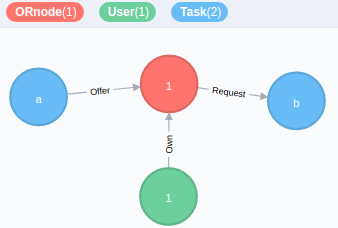
\includegraphics[]{example1.png}
  \caption{User 1 uploads an ORpair to offer task a and requests task b in exchange.}
  \label{example1}
\end{figure}

\begin{figure}
  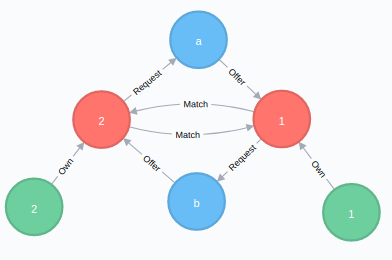
\includegraphics[]{example2.png}
  \caption{User 2 uploads an ORpair to offer task b and requests task a in exchange.
           \\Now there is a cycle/match.}
  \label{example2}
\end{figure}

An \textbf{offer network} instance can be formally modeled as a directed graph, $G$, where vertices $t \in T$ represent tasks, $u \in U$ users, and labeled directed edges $(t_a,t_b)$ represent an offer by user $u_1$ to do task $t_a$ in exchange requested task $t_b$. Due to implemention details in Neo4j\footnote{\url{https://neo4j.com/}}, (offer, request) nodes are created for labeled directed edges, called \textbf{ORpairs}. This is the \textbf{the task-centric model}\footnote{An alternative is an \textbf{ORpair-centric model} where each ORpair is directly linked to all offer or request compatible ORpairs.}.  See Figure \ref{example1}.

A matching of users who can satisfy each other is a vertex cycle. See the simplest case below in Figure \ref{example2}. There is a match acceptance probability $p$, which is assumed to be uniform and independent\footnote{Moreover, Dickerson \cite{Dick} notes this assumption potentially also protect users, such as badly sick patients, from being marginalized in addition to being simpler to analyze.}.

\subsection{Scale-Free Task Distribution}
The ReadItSwapIt data is scale-free. This means that for large degrees $k$, the fraction of nodes with degree k is proportional to $k^{-\gamma}$\footnote{\url{https://en.wikipedia.org/wiki/Scale-free_network}}. In colloquial terms, this means that a few tasks are very popular and most tasks are only offered or requested by a few users. There will likely be a small difference in \textit{offer} and \textit{request} popularity for tasks.

Worth mentioning on this note is a user-centric study of the eBay graph \cite{ebay}\footnote{The data is obtained via crawling eBay feedback.}. They noted the following properties on eBay:

\begin{itemize}
  \item Skewed degree distribution: i.e., there are a few big sellers.
  \item Dissasortativity: users tend to buy and sell different types of products.
  \item Linear preferential attachment in terms of positive feedback.
     \\ Strong aversion avoidance of users with negative feedback.
  \item Densification over time.
  \item No rich club connectivity (basically because big nodes are mass sellers).
\end{itemize}

Dissasortativity implies that there will be little clustering: there will be many ORpairs between diverse task types\footnote{The specialization of many exchange sites and services may seem to contradict this; however this may also be due to the ease of developing specialized mechanisms.}.

Densification over time implies new ORpairs are added at a faster rate than new tasks.

\subsubsection{Scale-Free Graph Model}
A modified a graph generator in NetworkX \cite{netX} is used to generate scale-free graphs, which is described by Bollobás, Borgs, Chayes, and Riordan in \textit{Directed Scale-Free Graphs} \cite{Bol}. It's a preferential attachment model.

The graph starts with a directed triangle.

Each time an edge\footnote{ORpair} is added, with probability
\begin{itemize}
  \item $\alpha$, create new node\footnote{task} $v$ and choose $w$ based on in-degree distribution.
  \item $\gamma$, create new node $w$ and choose $v$ based on out\_degree distribution.
  \item $\beta$, choose $v$ based on out-degree distribution and $w$ based on in-degree distribution.
\end{itemize}
Then add $(v,w)$ to the graph.

There are parameters $\delta_{in}$ and $\delta_{out}$ added to the degree so that nodes with zero degree are still chosen with non-zero probability. Let
$$c_1 = \frac{\alpha + \beta}{1 + \delta_{in}(\alpha + \gamma)} \mbox{ and } c_2 = \frac{\beta + \gamma}{1 + \delta_{out}(\alpha + \gamma)}$$
$$X_{IN} = 1 + 1/c_1 + c_2/c_1(\delta_{out} + 1_{\{\gamma \delta_{out}=0\}})$$
$$X_{OUT} = 1 + 1/c_2 + c_1/c_2(\delta_{in} + 1_{\{\alpha \delta_{out}=0\}})$$
$-X_{IN}$ and $-X_{OUT}$ are the power law exponents. Note that in this model in-degree and out-degree distributions are independent.

Thus with probability $p_d$ the directed scale-free graph generation is used, and with probability $1-p_d$ prefernetial attachment is done only with respect to total degree and $\frac{\delta_{in} + \delta_{out}}{2}$. The non-directed power law exponent is ???.

In my modification the model generates a set number of edges and for each edge adds a new task with probability $\alpha + \gamma$.

\subsection{Dynamic Offer Network Specification}
The dynamic offer network starts with a scale free graph generated as above with $N^o_0$ ORpairs and $N^u_0$ users and each time-step $t$, $n^o$ and $n^u$ new ORpairs and users. Each step there are $(\alpha + \gamma) n^o$ new tasks added to the network every step. The experiment is run until $N^o_m$ ORpairs have been added. Between each step matchings are suggested, processed (by users), and accepted ORpairs are removed from the graph.

It is possible to make $n^o$ and $n^u$ depend on $N^o_t$, $N^u_t$, on each other, or be drawn from a probability distribution.

\subsection{Cycle Size and Acceptance Probability}

\subsubsection{Motivation}
The optimal solution clearly depends on acceptance probability, primarily biased by the optimal cycle size. In general, finding a maximum edge-disjoint cycle cover with cycle-weights (to account for acceptance probability) is NP-hard \cite{Bir}, so the prefrred algorithm may depend on the current estimation for $p$. If near $1$, (near) unlimited cycle sizes are welcome; if low, 2-exchanges will always be preferable.  In the middle, an algorithm may want to choose cycles with greatest expected value.

Below I include some basic probabilistic anlaysis to find out how high is high and how low is low.

Similar analysis is done by Dickerson \cite{Dick} \cite{Dick3}; however, Dickerson uses an optimal solver and pays less attention to determining heuristics.

\subsubsection{Analysis}

In a cycle $c$ of size $k$, the probability of acceptance is $p_k = p^k$.

Thus the expected number of satisfied users is: $\E[c_k] = k p^k$. For a given $p$, the best cycle size is given by $k = -\frac{1}{\ln p}$, and the best attainable for $p$ is $-\frac{1}{e \ln p}$.

\begin{figure}
  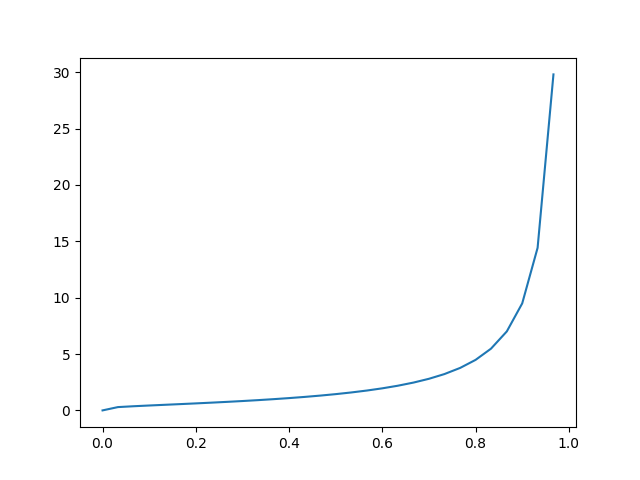
\includegraphics[scale=0.65]{best-k.png}
  \caption{Best k-cycle for p from 0.8 to 1}
  \label{best-k}
\end{figure}

\begin{figure}
  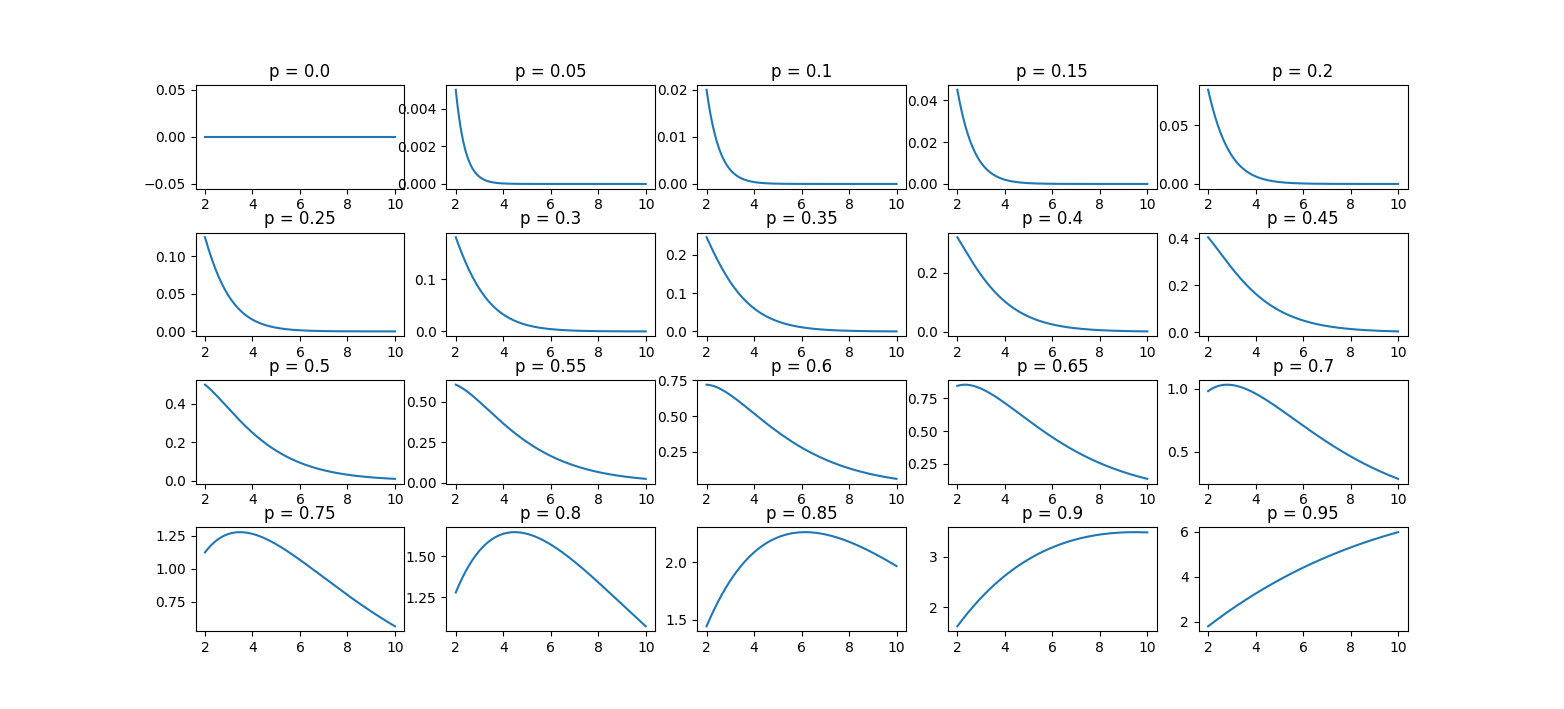
\includegraphics[width=\textwidth]{eckp1.png}
  \caption{$\E[c_k]$ for $k = 2 \dots 10$}
  \label{eckp1}
\end{figure}

\begin{figure}
  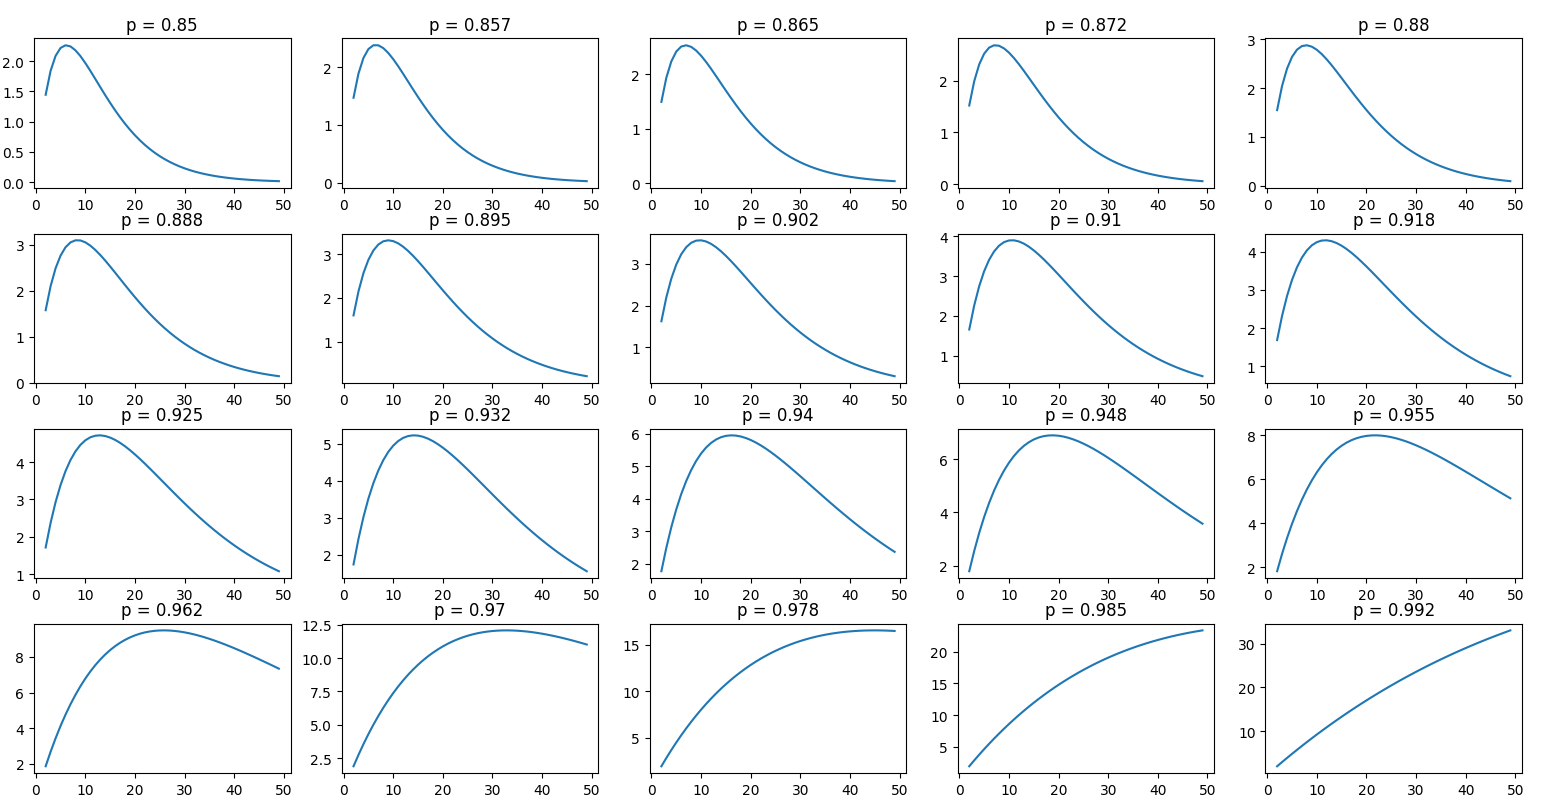
\includegraphics[width=\textwidth]{eckp2.png}
  \caption{$\E[c_k]$ for $k = 2 \dots 50$}
  \label{eckp2}
\end{figure}

As can be seen in Figure \ref{best-k}, the optimal cycle size exponentially incresaes for $p > 0.95$ ($k \approx 19.5$), so the maximum without cycle-length constraints will likely suffice. And in Figure \ref{eckp1} one sees that $2$-cycles are optimal $p < 0.7$. The Polynomial time solution is less clear for the following cases:
\begin{itemize}
  \item $0.7 < p < 0.85$ where $ 2 < k < 10$ is optimal.
  \item $0.85 < p < 0.95$ where $ 10 < k < 30$ is optimal,
      \\yet the larger cycles are little bitter than shorter ones.
\end{itemize}

For human users without very specific task formulations, $p$ likely lies in this range.

\subsubsection{How many matches are needed to for acceptance?}
There is an approach\footnote{The hanging ORpair approach is discussed in the Algorithms section.} to make long-cycles more feasible with moderate $p$ where a match can be accepted so long as both of its neighbors in a cycle accept the match as well. Thus we are interested in how many times a user needs to be matched before getting a satisfactory match.

In a given round, the probability the suggested match goes through is $p^3$ as both neighbors in a cycle also need to accept. Thus the expected number of rounds for acceptance follows the geometric distribution: $\sum_{k=0}^{\infty} k p^3 (1 - p^3)^{k-1} = \frac{1}{p^3}$.

\begin{figure}
  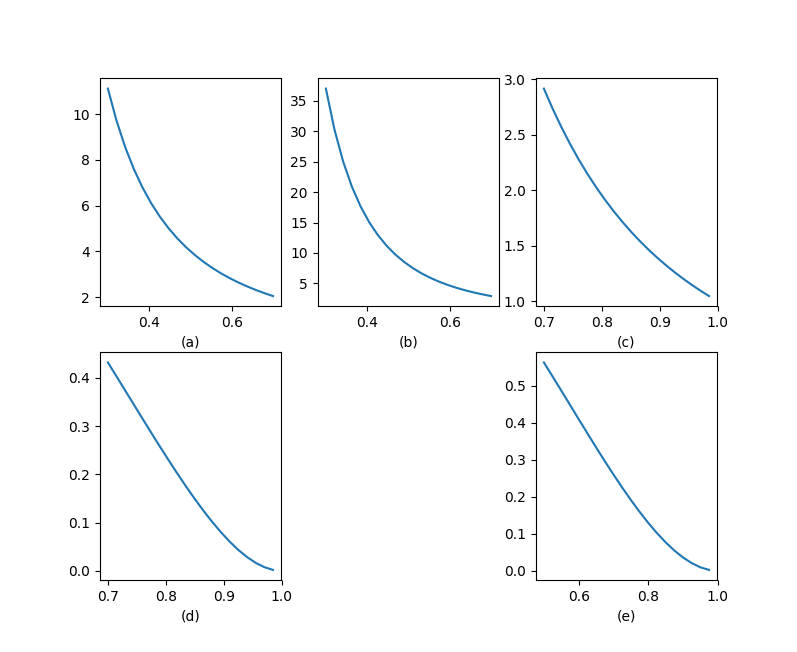
\includegraphics[width=\textwidth]{nrounds.png}
  \caption{(a)-(c) plot expected number of rounds for acceptance of an ORpair for different $p$. (a) is for 2-cyles. (b) and (c) k-cycle. (d)-(e) plot the probability of an ORpair not being accepted in 2 rounds. (d) is k-cycle and (e) is 2-cycle.}
  \label{nrounds}
\end{figure}

As one can see in Figure \ref{fig:nrounds}, one expects 5 rounds to be needed by $p = 0.6$. Fortunately, for $p > 0.7$, one expcets less than 3 rounds to be needed. With 2-cycles, one only needs 3 or 4 rounds for $p = 0.6$ or $0.5$. For lower $p$, the offer network will likely be too frustrating for human users: matching will have to be done on more detailed task specifications \footnote{Acceptance probaility is likely proportional to how detailed task specifications are; however, there are also limits as to how detailed humans can be.}.

One can also easily calculate the probability acceptance for an ORpair will take more than two rounds: $1 - (p^3 + p^3 * (1 - p^3))$.

\subsubsection{Application to Kidney Exchange}
When exchanging kidneys there is a type of incompatibility not checked prior to initial matching: PRA (percent reactive antibody). Roth et al. \cite{Rot2} split the distribution into low, medium, and high PRA with respective 5, 45, and 90 percent probability of positive crossmatch (rejection). The frequency among kidney donors is 70, 20, and 10 percent. Thus for 10 percent of matches, anything but 2-way has very low expectation, and for another 20 percent, 2-way is still expected to perform twice as well as 4-way matches. For the remaining 70 percent, however, 20-way matches are best, and 50-way still preferable to anything less than 10-way matches.

Thus when mixing low, medium, and high PRA the result of 2-way and 3-way matches being almost as good as unconstrained is unsurprising. This also seems to be a result of there only being 4 blood types, and thus no benefit to $(>4)$-way matches \cite{Rot2}.

Morevore, Dickerson \cite{Dick} \cite{Dick3} calculates acceptance probabiltiy\footnote{Optimistically based on only positive crossmatch.} to be at most $30$ percent: that is, 2-way matches always preferable to 3-way.

\subsection{Additional Features}

Below is a list of potentially desirable features of an offer network that don't qualify for an MVP:
\begin{itemize}
  \item Reputation biased matching
  \item Preferences for matching based on
    \begin{itemize}
      \item User preferences
      \item Task prefreences
    \end{itemize}
  \item ORs and ANDs of offers or request
  \item Task categories for hard/soft constraints
    \begin{itemize}
      \item Similarity based task-grouping
    \end{itemize}
\end{itemize}


\end{document}


%% For loading example graph into Neo4j
%%CREATE (t1:Task {id:'a'})
% CREATE (t2:Task {id:'b'})
% CREATE (u:User {id:'1'})
% CREATE (u2:User {id:'2'})
% CREATE (o:ORpair {id:'1', offer:'a', request:'b', user:'1'})
% CREATE (o2:ORpair {id:'2', offer:'b', request:'a', user:'2'})
% CREATE (t1)-[:Offer]->(o)-[:Request]->(t2)
% CREATE (t2)-[:Offer]->(o2)-[:Request]->(t1)
% CREATE (u)-[:Own]->(o)
% CREATE (u2)-[:Own]->(o2)

% Replacing:
%
% \begin{center}
  % \begin{tikzpicture}
    % \node[draw, circle] (ta) at (0,0) {$t_a$};
    % \node[draw, circle] (tb) at (6,0) {$t_b$};
    % \draw[-latex] (ta) to[bend left=10] node[above] {$u_1$} (tb);
    % \draw[-latex] (tb) to[bend left=10] node[below] {$u_2$ }(ta);
  % \end{tikzpicture}
% \end{center}
%
% \begin{center}
  % \begin{tikzpicture}
    % \node[draw, circle] (ta) at (0,0) {$t_a$};
    % \node[draw, circle] (tb) at (6,0) {$t_b$};
    % \path [->] (ta) edge node[above] {$u_1$} (tb);
  % \end{tikzpicture}
